%\part{Fundamentos Matem\'aticos}

%*****************************************
\chapter{Problemas, Algoritmos y Complejidad}\label{ch:preliminaresComputacion}
%*****************************************

% handbook of applied
% apuntes algebra conmutativa


%para relacionar con la criptografía, ver WIKIPEDIA
% https://en.wikipedia.org/wiki/Computational_complexity_theory#Problems_in_NP_not_known_to_be_in_P_or_NP-complete

% Handbook of applied
% Fundamentals of Computer Security
% Apuntes AED II

% Estructura:
% Intro con definiciones de problema, algoritmo, Problemas de decisión
%  Subsección: Notación asintótica, clases de complejidad (polinómico, exponencial, ejemplos)
%  Subsección: Clases P y NP, ___
%  Subsección: Algoritmos probabilísticos, ¿ensembles?, ¿preliminares de estadística?
%  Subsección: El uso en criptografía por la suposición de P!=NP, intractability, nombrar los 3 problemas NPI, y dejar el estudio y por qué son NPI para sus respectivas secciones.


En este capítulo introducimos unos preliminares sobre la complejidad computacional, que nos permitirán entender qué problemas matemáticos, y por qué, se utilizan en criptografía. Comencemos con unas definiciones:

\begin{definition}\index{Problema}
	Llamamos \textit{problema} a la descripción general de una tarea que depende de unos parámetros. La \textit{definición} de un problema consta de dos partes. La primera da el escenario del problema, describiendo los parámetros necesarios. La segunda parte indica una pregunta de la que se espera una respuesta o solución.
\end{definition}

\begin{example}
	Vamos a considerar el problema de multiplicar dos matrices. La definición del problema sería:

	\begin{tabular}{|ll}
		\textit{Nombre:} & Problema multiplicación de matrices. \\
		\textit{Parámetros:} & Dos matrices $A_1$ y $A_2$. \\
		\textit{Pregunta:} & ¿Cuál es la matriz $A$ tal que $A=A_1 \cdot A_2$? \\
	\end{tabular}
\end{example}

\begin{definition}\index{Instancia de un problema}
	Una \textit{instancia} de un problema es el caso particular de un problema al que se le han dado valores a los parámetros.
\end{definition}


\begin{definition}\index{Algoritmo}
	Un \textit{algoritmo} es una lista de instrucciones que para una instancia produce una respuesta correcta. Se dice que un algoritmo \textit{resuelve} un problema si devuelve respuestas correctas para todas las instancias del problema.
\end{definition}


\begin{definition}\index{Problema de decisi\'on}
	Se llama \textit{problema de decisión} a un problema cuya respuesta está en el conjunto $\mathcal{B}= \{Verdadero, Falso\}$.
\end{definition}

Asociado a un problema, podemos establecer un problema de decisi\'on que a veces
puede resultar de una dificultad muy diferente del problema original. Consideremos el siguiente problema de decisi\'on asociado al problema planteado del producto de matrices:

\begin{example}

	\begin{tabular}{|ll}
		\textit{Nombre:} & Problema de decisi\'on de multiplicación de matrices. \\
		\textit{Parámetros:} & Tres matrices $A$, $A_1$ y $A_2$. \\
		\textit{Pregunta:} & ¿$ A = A_1 \cdot A_2$? \\
	\end{tabular}
	\\
	\hfil

	Un algoritmo para solucionarlo ser\'ia realizar el producto de las matrices $A_1$ y $A_2$ y comprobar que el resultado coincide con $A$. Esto nos dar\'ia una soluci\'on del problema por reducci\'on al caso anterior y por lo tanto la dificultad del problema ser\'ia la misma que la del problema original.

	Sin embargo, podemos encontrar en algunos casos algoritmos m\'as eficientes que nos permitan resolver el problema de decisi\'on pero que no establecen una soluci\'on al problema inicial.
\end{example}

Este ejemplo de la multiplicaci\'on de matrices, lo trataremos m\'as adelante, pero se puede entender la diferencia fundamental que puede suponer la informaci\'on adicional que nos ha ofrecido el nuevo problema con otro ejemplo. Mientras que dado un n\'umero, determinar cuales son sus factores es un problema muy dif\'icil, el problema de determinar si un factor concreto es un divisor de un n\'umero es tan simple como hacer una divisi\'on.

Todos estos ejemplos los trataremos m\'as en profundidad a lo largo de la memoria, pero antes de seguir adelante vamos a introducir m\'as formalmente el concepto de complejidad.

\hfil

\section{Notación asintótica}

Para poder estudiar cómo crecen el tiempo de ejecución, la memoria usada, o cualquier otro recurso, de un algoritmo, dependiendo del tamaño de los datos de entrada, utilizamos distintas \textit{notaciones asintóticas}. Nos interesa en particular la siguiente:

\begin{definition}\index{O grande}\index{Orden (de complejidad)}
	Sea $f : \mathbb{N} \rightarrow \mathbb{R}^+$. Definimos la notación \textit{O grande} u \textit{orden} de $f$ al conjunto de funciones de $\mathbb{N}$ a $\mathbb{R}^+$ acotadas superiormente por un múltiplo positivo de $f$ a partir de cierto valor $n \in \mathbb{N}$:

	$O(f) = \{t:\mathbb{N} \rightarrow \mathbb{R}^+ \, | \; \exists c \in \mathbb{R}^+,\, \exists
	n_0\in \mathbb{N} \, : \, t(n) \leq c\cdot f(n) \quad \forall n \geq n_0  \}$.

\end{definition}

\hfil

Para estudiar el tiempo de ejecución, $t : \mathbb{N} \rightarrow \mathbb{R}^+$ (el tiempo promedio, el caso más desfavorable, \dots), de un algoritmo, buscaremos una función $f$ que acote a $t$ lo más de cerca posible. Para ello definimos la relación de orden:

\begin{definition}
	Sean $f, g : \mathbb{N} \rightarrow \mathbb{R}^+$.
	%\marginpar{Comparación de órdenes: $ O(1) \leq O(ln\,n) \leq O(\sqrt{n}) \leq O(n) \leq O(n\,ln\,n) \leq O(n^c) \leq O(n^{ln\,n}) \leq O(c^n) \leq O(n!) \leq O(n^n) $, donde $c>1$ constante.}
	Diremos que  $O(f) \leq O(g)$ si $\forall t \in O(f)$ se tiene que $t \in O(g)$, es decir,  $O(f) \subseteq O(g)$.
\end{definition}

Para acotar $t$ buscaremos el menor $O(f) : t\in O(f)$.

% La función $t : \mathbb{N} \rightarrow \mathbb{R}^+$, del tiempo de ejecución de un algoritmo, toma en general como parámetro el tamaño de la entrada. Éste depende de la representación que se le dé a los parámetros, pero podemos pensar siempre en la representación binaria de los números enteros excepto que se indique lo contrario. Esta representación utiliza $1+log_2(n)$ bits para un entero $n$, y podemos simplificar para $n$ suficientemente grande a $log_2(n)$.

\hfill
\section{Algoritmos Polinomiales, Exponenciales y Subexponenciales}

Antes de empezar a ver los tipos de algoritmos, es interesante ver un ejemplo. Pensemos en el algoritmo tradicional de suma de dos n\'umeros decimales que por simplicidad
consideraremos que tienen el mismo n\'umero de cifras $l$. Si repasamos este algoritmo, lo que tenemos que hacer es ir sumando una a una cada cifra de los dos n\'umeros teniendo
en cuenta si nos llevamos algo de la operaci\'on anterior. Esto nos da un n\'umero de operaciones que es esencialmente $l$, o $2l$ si consideramos tambi\'en la correcci\'on dependiente
de la suma anterior.

Un algoritmo como este es muy efectivo puesto que aunque los n\'umeros involucrados tengan 8 \'o 10 cifras, un ni\~no en la escuela puede hacerlo sin dificultad en un tiempo relativamente corto.

El algoritmo de la multiplicaci\'on ya es un poco m\'as complicado, puesto que tenemos que multiplicar cada una de las cifras del primer n\'umero por cada una de las cifras del segundo
y luego sumar, eso nos da un n\'umero de operaciones dependientes de $l^2$ y no de $l$ como antes, pero aun as\'i el algoritmo es f\'acil de hacer con papel y l\'apiz si no superamos
las 4 \'o 5 cifras.

Sin embargo, pensemos en el algoritmo para el c\'alculo del factorial, el n\'umero de operaciones ahora no depende de $l$, el número de cifras, sino de el valor del n\'umero, pues si estamos hablando de la base $10$, ser\'ian
$10^l$ el n\'umero aproximado de multiplicaciones que tendr\'iamos que hacer. Esto ser\'ia totalmente imposible hacerlo con l\'apiz y papel para valores tan peque\~nos como $l = 3$
porque requerir\'ian un n\'umero entre $100$ y $999$ multiplicaciones.

Cuando el tiempo que tarde un algoritmo depende de una potencia del n\'umero de cifras de la entrada (lo que se suele llamar del tama\~no de la entrada) diremos que el algoritmo es polin\'omico, en el ejemplo anterior, la suma depende de $l$ y el producto de $l^2$.
Pero si el tiempo depende del valor concreto del n\'umero como en el caso del factorial diremos que el algoritmo es exponencial.

Vamos a formalizar estos conceptos utilizando la notaci\'on asint\'otica. Para ello empecemos fij\'andonos que el n\'umero de cifras en base $b$ de un n\'umero $n$ es
$\log_b(n) = \ln(n)/\ln(b)$ por lo que cambiar de base \'unicamente nos modifica una constante, que en la notaci\'on asint\'otica se desprecia, es decir $\log_b(n) \in O(\ln(n))$.

Podemos decir por tanto que el tama\~no de un n\'umero es del orden $\ln(n)$ puesto que sea la que sea la base con la que trabajemos, la diferencia ser\'a una constante.

\begin{definition}\index{Algoritmo polinomial}\index{Algoritmo exponencial}
Se llama algoritmo de \textit{tiempo de cálculo polinomial} al algoritmo cuya función de tiempo del caso más desfavorable es de orden
$O(l^k)$, donde $l$ es el tamaño de la entrada y $k$ una constante. Si la entrada es num\'erica, tal y como hemos visto $l$ se puede tomar $\ln(n)$.
Cualquier algoritmo cuyo tiempo de ejecución no puede acotarse de esa manera se llama de \textit{tiempo de cálculo exponencial}.
\end{definition}

En los problemas que trataremos en esta memoria, aparecen algoritmos que no siendo polin\'omicos, tampoco son puramente exponenciales.
Estos son conocidos como algoritmos subexponenciales y vendr\'an dados por un par\'ametro $\alpha$ que de forma cont\'inua nos dar\'a una cierta
medida de la complejidad.

\begin{definition}\index{Algoritmo subexponencial}
Sea $\alpha$ un n\'umero real en el intervalo $[0,1]$ y sea $c$ un n\'umero real positivo. Llamaremos funci\'on subexponencial de par\'ametros
$\alpha$ y $c$ a la funci\'on
\[ L_n[\alpha,c] = e^{c(\ln n)^\alpha (\ln \ln n)^{1-\alpha}} \]
\end{definition}

Esta notaci\'on tiene dos casos extremos, que son el caso $\alpha = 0$ que nos proporciona las funciones $L_n[0,c] = e^{c(\ln\ln n)} =(\ln n)^c$ y el
caso $\alpha = 1$ que nos da $L_n[1,c] = e^{c(\ln n)} = n^c$. Por lo tanto, un algoritmo que nos de un tiempo de ejecuci\'on $O(L_n[0,c])$ es un
algoritmo polin\'omico, mientras que uno que nos de un tiempo de ejecuci\'on $O(L_n[1,c])$ es puramente exponencial.

Estrictamente hablando, cuando $\alpha \not= 0$ la complejidad se considera exponencial, pero
sin embargo este par\'ametro $\alpha$ puede tomar muchos valores intermedios y ser\'a \'util para precisar la complejidad
de algunos algoritmos.

\section{Clases de complejidad}
\index{Clase de complejidad}

Tal y como hemos visto en la secci\'on anterior, un algoritmo se denomina de complejidad {\em polin\'omica}
cuando la función de tiempo del caso más desfavorable es de orden $O(l^k)$, donde $l$ es el tamaño de la entrada y $k$ una constante.

A veces se denominan \textit{buenos} o \textit{eficientes} a los algoritmos polinomiales, e \textit{ineficientes} a los exponenciales, siendo los subexponenciales una soluci\'on intermedia.
Estas propiedades dependen de la notaci\'on asint\'otica, sin embargo, hay que hacer algunas consideraciones. Por un lado est\'an las
constantes ocultas, aunque la notaci\'on asint\'otica nos diga que es lo mismo que la complejidad sea $l^3$ que $10^{20} l^3$, la constante oculta $10^{20}$
puede generar importantes diferencias. Por otro lado, especialmente en criptograf\'ia, los tama\~nos con los que nos movemos no
suelen variar demasiado, y debemos ser conscientes de que un algoritmo exponencial puede llegar a ser m\'as eficiente que uno polin\'omico para valores peque\~nos de $l$.

A pesar de estas puntualizaciones que podr\'iamos hacer en casos concretos y que trataremos a lo largo de esta memoria, podemos considerar que la
notaci\'on asint\'otica es una buena medida para el estudio de la complejidad de los algoritmos.

Bas\'andonos en esta notaci\'on asint\'otica, podemos definir las siguientes clases de complejidad en problemas de decisi\'on:

\begin{definition}\index{P}
	El conjunto de problemas de decisión que se pueden resolver en tiempo polinomial se llama clase \textbf{P}.
\end{definition}

\begin{definition}\index{NP}
	\label{def:NP}
	Se llama clase de complejidad \textbf{NP} al conjunto de problemas de decisión
	donde una respuesta que sea $Verdadero$ se puede verificar en tiempo polinomial,
	dada cierta información extra, que llamaremos {\em certificado} o {\em testigo}
	\footnote{Utilizaremos certificado y testigo como traducci\'on de {\em certificate} y {\em witness}.
	Dependiendo del contexto se suele usar un nombre u otro, incluso a veces se considera
	que dicha informaci\'on adicional es el {\em secreto} al que se refieren las pruebas
	de conocimento cero.}.
\end{definition}

%\begin{definition}
%	Se llama clase de complejidad \textbf{co-NP} al conjunto de problemas de decisión
%	donde una respuesta que sea $Falso$ se puede verificar en tiempo polinomial,
%	dado el correspondiente \textit{certificado}.
%\end{definition}

Es inmediato que  que \textbf{P} $\subseteq$ \textbf{NP}.% y \textbf{P} $\subseteq$ \textbf{co-NP}.

\begin{example}[Problema en \textbf{NP}]
	Consideremos el siguiente problema de decisión:

	\begin{tabular}{|ll}
		\textit{Nombre:} & Problema del entero compuesto. \\
		\textit{Parámetros:} & Un entero positivo $n$. \\
		\textit{Pregunta:} & ¿Es $n$ compuesto? Es decir, ¿existen \\
		&  enteros $a$, $b > 1$ tal que $n=ab$? \\
	\end{tabular}
	\\

	El problema pertenece a \textbf{NP} porque se puede comprobar en tiempo polinomial que
	$n$ es compuesto si nos dan su \textit{certificado}, un divisor $a$ de $n$, tal que $1 < a < n$.
	Basta usar la división euclídea de $n$ entre $a$ y ver que el resto es $0$. Sin embargo,
	aún no se conoce si el problema pertenece a \textbf{P}.
\end{example}


\hfil

\begin{definition}\index{Reducible en tiempo polinomial}
	\label{reducePoly:def}
	Sean dos problemas de decisión $L_1, L_2 \in $ \textbf{NP}, con correspondientes
	conjuntos de instancias $I_1$ e $I_2$. Sean $I_1^+$ e $I_2^+$ los subconjuntos
	de todas las instancias ``$Verdaderas$'' de $I_1$ e $I_2$, respectivamente.
	Decimos que $L_1$ es \textit{reducible en tiempo polinomial} a $L_2$, $L_1
	\leq_P L_2$, si existe una función $f:I_1 \Rightarrow I_2$ que cumple:

	\begin{enumerate}
		\item Es ejecutable en tiempo polinomial.
		\item $x \in I_1^+  \Leftrightarrow  f(x) \in I_2^+ $.
	\end{enumerate}
\end{definition}

\hfil

De manera más informal, se dice que $L_1$ se reduce en tiempo polinomial a
$L_2$ si hay un algoritmo que resuelve $L_1$ utilizando como subrutina un
algoritmo que resuelve $L_2$, y que se ejecuta en total en tiempo polinomial,
si lo hace el algoritmo que resuelve $L_2$.

Si $L_1 \leq_P L_2$, entonces se puede entender que $L_2$ es, al menos
computacionalmente, tan difícil como $L_1$, o que $L_1$ no es más difícil que $L_2$.

\begin{definition}\index{NP-completo}\index{NPC}
	Un problema de decisión $L$ se dice que es \textbf{NP}-completo, o \textbf{NPC} si:
	\begin{enumerate}[label=(\roman*)]
		\item $L \in $ \textbf{NP}, y
		\item $L_1 \leq_P L \quad \forall L_1 \in $ \textbf{NP}.
	\end{enumerate}
\end{definition}

\hfil

Los problemas \textbf{NPC} son los más difíciles entre los \textbf{NP}
en el sentido de que son al menos tan difíciles como el resto de
problemas en \textbf{NP}.

Una pregunta que nos puede aparecer es si realmente existen estos problemas de
tipo \textbf{NPC}. En este caso la respuesta es afirmativa, dichos problemas
existen y basta con encontrar uno de ellos.
Veamos el problema \textbf{NPC} más característico:

\begin{tabular}{|ll}
	\textit{Nombre:} & Problema de satisfacibilidad booleana (SAT). \\
	\textit{Parámetros:} & Una colección finita $C$ de expresiones booleanas \\
	&  con variables y sin cuantificadores. \\
	\textit{Pregunta:} & ¿Hay alguna asignación de las variables que \\ & haga $Verdadero$ a $C$? \\
\end{tabular}
\\

\begin{theorem}[Teorema de Cook (1971)]
	El problema de satisfacibilidad booleana es \textbf{NPC}.
\end{theorem}
%\marginpar{Para conocer más sobre el problema y la demostración se puede consultar \citep{book:1056906}.}

O expresado de otra manera:

\begin{theorem}
	\label{redNPC:theo}
	Todo problema $Q \in $ \textbf{NP} se puede reducir en tiempo polinomial al problema de satisfacibilidad booleana: $\forall Q \in $ \textbf{NP}, $Q \leq_P SAT$.
\end{theorem}


\hfil

Existen otros problemas del tipo \textbf{NPC} que nos aparecer\'an m\'as adelante,
como el de la 3-coloraci\'on de grafos, pero la existencia de uno es suficiente
por la equivalencia te\'orica de todos ellos.

%%%%%%%%%%%%%%
%A día de hoy conocemos ciertas propiedades sobre las clases de equivalencia, pero
%quedan muchas cuestiones sin resolver:
%
%\begin{itemize}
%	\item Uno de los siete problemas del milenio, ¿\textbf{P} $=$ \textbf{NP}?
%	\item ¿\textbf{NP} $=$ \textbf{co-NP}?
%	\item ¿\textbf{P} $=$ \textbf{NP} $\cap$ \textbf{co-NP}?
%\end{itemize}
%%%%%%%%%%%%%%%

A día de hoy conocemos ciertas propiedades sobre las clases de equivalencia, pero
quedan muchas cuestiones sin resolver, entre ellas, uno de los siete problemas del milenio, ¿\textbf{P} $=$ \textbf{NP}?

La opinión de los expertos en base a ciertas evidencias es que la respuesta a
las tres es \textit{no}, pero hasta que se encuentren demostraciones formales
de cada una, quedarán en conjeturas. Y basándose en esas conjeturas es donde
se apoya la seguridad informática.


%\begin{figure}[bth]
%	\begin{center}
%		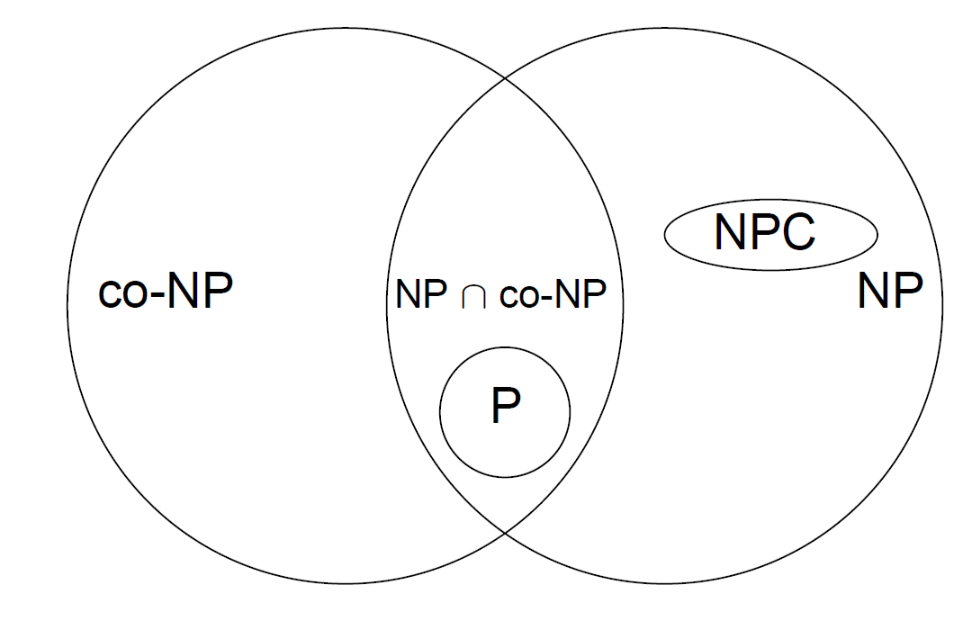
\includegraphics[width=.45\linewidth]{gfx/NPclasses}
%	\end{center}
%	\caption{Conjetura de las relaciones entre clases \textbf{NP}, \textbf{co-NP},
%	\textbf{NPC}, \textbf{P}.}
%	\label{fig:NPclasses}
%\end{figure}


Existen tres problemas que se conoce que pertenecen a \textbf{NP}, pero se
desconoce a día de hoy si pertenecen a \textbf{P} o \textbf{NPC}: el
isomorfismo de grafos, el logaritmo discreto y la factorización de enteros.

En los siguientes capítulos los estudiaremos como base de diferentes pruebas
de conocimiento cero.




\section{Algoritmos probabilísticos}

\index{Algoritmo probabil\'istico}

Para intentar resolver la infactibilidad computacional de ciertos problemas, surge un modelo alternativo de computación que utiliza métodos probabilísticos. Estos métodos no pueden asegurar cotas superiores absolutas de tiempo, e incluso pueden devolver una respuesta errónea. Sin embargo, dadas unas cotas muy pequeñas de errores, en la práctica, ciertos métodos probabilísticos son más eficientes que los algoritmos conocidos, pues el tiempo de ejecución \textit{esperado} del método, calculado probabilísticamente, es menor que el orden del algoritmo original.


% Tipos de algoritmos probabilísticos según errores
% Ejemplo de test de primalidad

\begin{definition}\index{Monte Carlo}
	Llamamos \textit{algoritmo de Monte Carlo} a un algoritmo probabilístico que resuelve un problema de decisión, pero tiene un error $\epsilon$ de equivocarse.

	Decimos que es \textit{parcialmente} $Verdadero$ si cuando se le da una instancia $Verdadera$ nunca se equivoca, pero si la instancia es $Falsa$ puede devolver $Verdadero$ con probabilidad $\epsilon$. De la misma manera, decimos que es \textit{parcialmente} $Falso$ si siempre resuelve correctamente instancias $Falsas$, pero puede cometer un error al resolver instancias $Verdaderas$.
\end{definition}


\begin{definition}\index{Las Vegas}
	Llamamos \textit{algoritmo de Las Vegas} a un algoritmo probabilístico que resuelve un problema de decisión, pero o bien lo resuelve correctamente, o bien informa de error y termina sin resolver el problema con una probabilidad $\epsilon$.
\end{definition}

Un problema que es tratado en muchos textos como un problema probabil\'istico aunque hoy en d\'ia ya no es un ejemplo v\'alido es el de la primalidad. Vamos a exponerlo porque tambi\'en nos servir\'a para explicar algunos otros aspectos de la complejidad de algoritmos.

\begin{example}[Test de primalidad]
	El problema de decisión:

	\begin{tabular}{|ll}
		\textit{Nombre:} & Problema de primalidad (PRIM). \\
		\textit{Parámetros:} & Un entero $n$. \\
		\textit{Pregunta:} & ¿Es $n$ primo? \\
	\end{tabular}
	\\
	\hfil
\end{example}

Este problema ha sido tratado tradicionalmente como un problema de tipo \textbf{NP} aunque en el a\~no 2002 se encontr\'o un algoritmo determinista de tiempo polin\'omico que resolv\'ia el problema. Este algoritmo se conoce como AKS por el nombre de sus descubridores, M. Agrawal, N. Kayal y N. Saxena. A pesar de ser un algoritmo polin\'omico, su compejidad te\'orica es del orden $O((log\, n)^{12+\epsilon})$, ver \citep[Página 314]{Pardo}, lo cual es muy ineficiente para el tama\~no de enteros que se utilizan en la
pr\'actica.

Existe sin embargo un algoritmo muy conocido de tipo probabil\'istico que nos determina si un entero es compuesto con total seguridad o primo con una probabilidad de error tan peque\~na como deseemos, es el algoritmo de Miller-Rabin. Este algoritmo es el que se sigue usando para las aplicaciones pr\'acticas puesto que el error que puede ofrecer puede hacerse tan peque\~no que sea incluso menor que el de un error en el hardware.

Otro ejemplo que podemos considerar para ver la diferencia entre un algoritmo determinista y uno probabil\'istico es el del producto de matrices. Dadas dos matrices $A_1$ y $A_2$ determinar si una tercera matriz $A$ es el producto de las dos anteriores.

Una soluci\'on al problema es hacer el producto y comprobar que el resultado es igual a $A$. Utilizando el algoritmo tradicional de multiplicaci\'on de matrices, la complejidad de este algoritmo ser\'ia $n^3$ si consideramos, para simplificar, matrices cuadradas de tama\~no $n$.  Existen algoritmos de multiplicaci\'on algo m\'as eficientes, pero vamos a ver c\'omo se podr\'ia resolver el problema utilizando un algoritmo probabil\'istico.

Si el producto de dos matrices $A_1 A_2$ es distinto de $0$, sabemos que el n\'ucleo de la aplicaci\'on lineal que representa dicho producto es de dimensi\'on como m\'aximo $n-1$, por lo que el n\'umero de vectores $X$ en el n\'ucleo es como m\'aximo $|K|^{n-1}$ siendo $|K|$ el n\'umero de elementos del cuerpo. La probablidad de que el vector $X$ est\'e en el n\'ucleo si este producto de matrices es distinto de $0$ es por lo tanto menor que $\frac{1}{|K|}$. Eligiendo aleatoriamente vectores $X_1, X_2, ..., X_t$ y comprobando que $A_1 (A_2 X_i)-A=0$ (lo cual puede hacer con complejidad $n^2$ si se hace en este orden) podemos obtener un algoritmo probabil\'istico de complejidad cuadr\'atica y con un error menor que $\frac{1}{|K|^t}$, valor que se puede hacer tan peque\~no como queramos de forma bastante r\'apida.
